%\documentclass[answers]{exam}
\documentclass{exam}
\usepackage{../../../mypackages}
\usepackage{../../../macros}
\geometry{a4paper, margin=2.5cm}

\SolutionEmphasis{\color{blue}}
\renewcommand{\solutiontitle}{\noindent}

\title{Exercice : Étude de fonction polynôme}
\author{N. Bancel}
\date{28 Mars 2025}
\begin{document}

\maketitle

\section*{Exercice : Étude des variations d’un polynôme }

\begin{questions}

\question Soit la fonction $g(x) = x^2 - 4x + 1$. Calculer l’expression de la dérivée de $g$.
\begin{solution}
La dérivée de $g$ est :
\[
g'(x) = 2x - 4
\]
\end{solution}

\question Étudier le signe de la dérivée de $g$ (on pourra dresser un tableau de signes).
\begin{solution}
On cherche à résoudre l’équation :
\[
g'(x) = 2x - 4 = 0 \Rightarrow x = 2
\]
$g'$ est une fonction affine de coefficient directeur positif ($a = 2 > 0$), donc :
\[
\begin{cases}
\forall x < 2, \quad g'(x) < 0 \\
\forall x > 2, \quad g'(x) > 0
\end{cases}
\]

\begin{center}
\begin{tikzpicture}
\tkzTabInit{$x$ / 1 , $g'(x)$ / 1}{$-\infty$, 2, $+\infty$}
\tkzTabLine{, -, z, +, }
\end{tikzpicture}
\end{center}
\end{solution}

\question En déduire le sens de variation de la fonction $g$.
\begin{solution}
On utilise les propriétés suivantes :
\begin{itemize}
\item $g'(x) < 0$ $\Rightarrow$ $g$ décroissante.
\item $g'(x) > 0$ $\Rightarrow$ $g$ croissante.
\item $g'(x) = 0$ $\Rightarrow$ extremum local.
\end{itemize}

Donc :
\begin{itemize}
\item $g$ est décroissante sur $]-\infty, 2[$
\item $g$ est croissante sur $]2, +\infty[$
\item $g$ atteint un minimum local en $x = 2$
\end{itemize}

Calculons $g(2)$ :
\[
g(2) = 2^2 - 4 \cdot 2 + 1 = 4 - 8 + 1 = -3
\]

\begin{center}
\begin{tikzpicture}
\tkzTabInit[lgt=2.5]
{$x$ / 1 , $g'(x)$ / 1 , $g(x)$ / 2}{$-\infty$, $2$, $+\infty$}
\tkzTabLine{, -, z, +, }
\tkzTabVar{+/ , -/$-3$ , +/ }
\end{tikzpicture}
\end{center}
\end{solution}

\question Déterminer le taux d’accroissement de la fonction $g$ entre $0$ et $3$.
\begin{solution}
Le taux d'accroissement est donné par :
\[
\frac{g(3) - g(0)}{3 - 0}
\]
Calculons :
\[
g(0) = 0^2 - 4 \cdot 0 + 1 = 1 \quad ; \quad g(3) = 3^2 - 4 \cdot 3 + 1 = 9 - 12 + 1 = -2
\]
\[
\Rightarrow \frac{-2 - 1}{3} = \frac{-3}{3} = -1
\]

\textbf{Conclusion :} Le taux d’accroissement de $g$ entre $0$ et $3$ est égal à $-1$.
\end{solution}

\question Tracer la courbe représentative de $g$.

\question Quelle est l’interprétation graphique du taux de variation calculé à la question précédente ? Cette interprétation est-elle bien vérifiée sur la figure tracée ?
\begin{solution}
Le taux d’accroissement représente le \textbf{coefficient directeur} de la droite sécante entre les points $A(0, g(0))$ et $B(3, g(3))$ :
\[
A(0, 1), \quad B(3, -2), \quad \Rightarrow \frac{-2 - 1}{3 - 0} = -1
\]

\textbf{Interprétation graphique :} Entre $x = 0$ et $x = 3$, la courbe de $g$ descend en moyenne de 1 unité en ordonnée pour chaque unité en abscisse.

\textbf{Sur le graphique :} Cette tendance est visible à travers l'inclinaison de la courbe entre les deux points.
\end{solution}

\end{questions}

\end{document}
